\documentclass[final,t]{beamer}
\mode<presentation>{\usetheme{PICB}}

% additional settings
\setbeamerfont{itemize}{size=\normalsize}
\setbeamerfont{itemize/enumerate body}{size=\normalsize}
\setbeamerfont{itemize/enumerate subbody}{size=\normalsize}

% additional packages
\usepackage{times}
\usepackage{amsmath,amsthm, amssymb, latexsym}
\usepackage{exscale}
%\boldmath
\usepackage{booktabs, array}
%\usepackage{rotating} %sideways environment
\usepackage[english]{babel}
\usepackage[latin1]{inputenc}
%\usepackage[orientation=portrait,size=a1]{beamerposter}
\usepackage[orientation=portrait,size=custom,width=59,height=84,scale=1]{beamerposter}
\listfiles
\graphicspath{{figures/}}
% Display a grid to help align images
% \beamertemplategridbackground[1cm]

\title{A Unifying Theory for\\[0.4ex]Experimental Symbolomics}

\author[Sample et al.]{John Sample, Mike Test and Mary Try}

\institute[PICB Shanghai]{Research Group for Experimental Symbolomics\\[0.4ex]
CAS-MPG Partner Institute and Key Laboratory for Computational Biology\\[0.4ex]
Shanghai Institutes for Biological Sciences, Shanghai, China}

\date[Aug. 31 , 2009]{Aug. 31 , 2009}

\newcommand{\footlinetext}{Contact: \{johnsample,miketest,marytry\}@picb.ac.cn \hskip2cm WWW: http://www.picb.ac.cn/Symbolomics}

% abbreviations
\usepackage{xspace}
\makeatletter
\DeclareRobustCommand\onedot{\futurelet\@let@token\@onedot}
\def\@onedot{\ifx\@let@token.\else.\null\fi\xspace}
\def\eg{{e.g}\onedot} \def\Eg{{E.g}\onedot}
\def\ie{{i.e}\onedot} \def\Ie{{I.e}\onedot}
\def\cf{{c.f}\onedot} \def\Cf{{C.f}\onedot}
\def\etc{{etc}\onedot}
\def\vs{{vs}\onedot}
\def\wrt{w.r.t\onedot}
\def\dof{d.o.f\onedot}
\def\etal{{et al}\onedot}
\makeatother

\begin{document}

\begin{frame}{} 

  \begin{columns}[t]    %%%%%%%%%%%%%%%%%%%%%%%%%%%%%%%%%%%%%%

    \begin{column}{.45\linewidth}
      \begin{block}{Overview}
        Sample poster with a more flexible/complex/interesting
        variant of the basic layout.
      \end{block}
    \end{column}

    \begin{column}{.45\linewidth}
      \begin{block}{Introduction}
        \begin{itemize}
        \item automatic sign language recognition system                                    %what
        \item \alert{necessary for communication} between deaf and
          hearing people
        \item \alert{continuous} sign language recognition,
          \alert{several} speakers, \alert{vision-based} approach, \alert{no
            special hardware}
        \item large vocabulary speech recognition (LVSR) system to
          obtain a textual representation of the signed
          sentences 
        \item evaluation of speech recognition techniques on \alert{publicly
          available sign language
          corpus}
        \end{itemize}
      \end{block}
    \end{column}
  \end{columns}    %%%%%%%%%%%%%%%%%%%%%%%%%%%%%%%%%%%%%%

  \begin{columns}[t]    %%%%%%%%%%%%%%%%%%%%%%%%%%%%%%%%%%%%%%
    \begin{column}{.7\linewidth}
      \begin{block}{Automatic Sign Language Recognition (ASLR)}

        \begin{columns}[T]    %--------------------------------
          \begin{column}{.49\linewidth}
            \begin{itemize}
            \item \alert{similar to speech recognition}: temporal sequences of images
            \item important features
              \begin{itemize}
              \item hand-shapes, facial expressions, lip-patterns
              \item orientation and movement of the hands, arms or body
              \end{itemize}
            \item HMMs are used to compensate time and amplitude variations of the signers\par
              \vskip2ex              
            \end{itemize}
          \end{column}
          \begin{column}{.49\linewidth}
            \begin{itemize}
            \item \alert{goal:} find the model which best expresses the observation sequence
            \end{itemize}
            \vskip2ex
          \end{column}
        \end{columns}    %--------------------------------
      \end{block}

      \begin{block}{Experimental Setup}
        \begin{columns}[t]    %--------------------------------
          \begin{column}{.5\linewidth}
            \noindent{\hskip1cm\textbf{Database}}
            \begin{itemize}
            \item system evaluation on the RWTH-BOSTON-104 database
              \begin{itemize}
              \item \alert{201 sentences} (161 training and 40 test sequences)
              \item vocabulary size of \alert{104 words}
              \item 3 speakers (2 female, 1 male)
              \item corpus is annotated in glosses
              \end{itemize}
            \end{itemize}

            \vskip1ex            
            \noindent{\hskip1cm\textbf{Problems}}
            \begin{itemize}
            \item 26\% of the training data are \alert{singletons}
            \item simple sentence structure
            \item one out-of-vocabulary (OOV) words with whole-word models
            \end{itemize}

            \vskip1ex            
            \noindent{\hskip1cm\textbf{Differences in Comparison to ASR}}
            \begin{itemize}
            \item simultaneousness                       % multi-channel ... but unclear if necessary
            \item signing space                          % verb flexion, negation, ... 
            \item environment                            % cluttered background, clothes, lighting, ... different microphones in ASR?
            \item speakers and dialects                  % as in ASR 
            \item coarticulation and movement epenthesis % 
            \item silence                                % unclear as there might be no energy changes in signal but still information, e.g. holded signs
            \item whole-word models and sub-word units   % necessary for large-vocabulary systems
            \end{itemize}
          \end{column}

          \begin{column}{.5\linewidth}
            \vskip0ex
            \centering    
            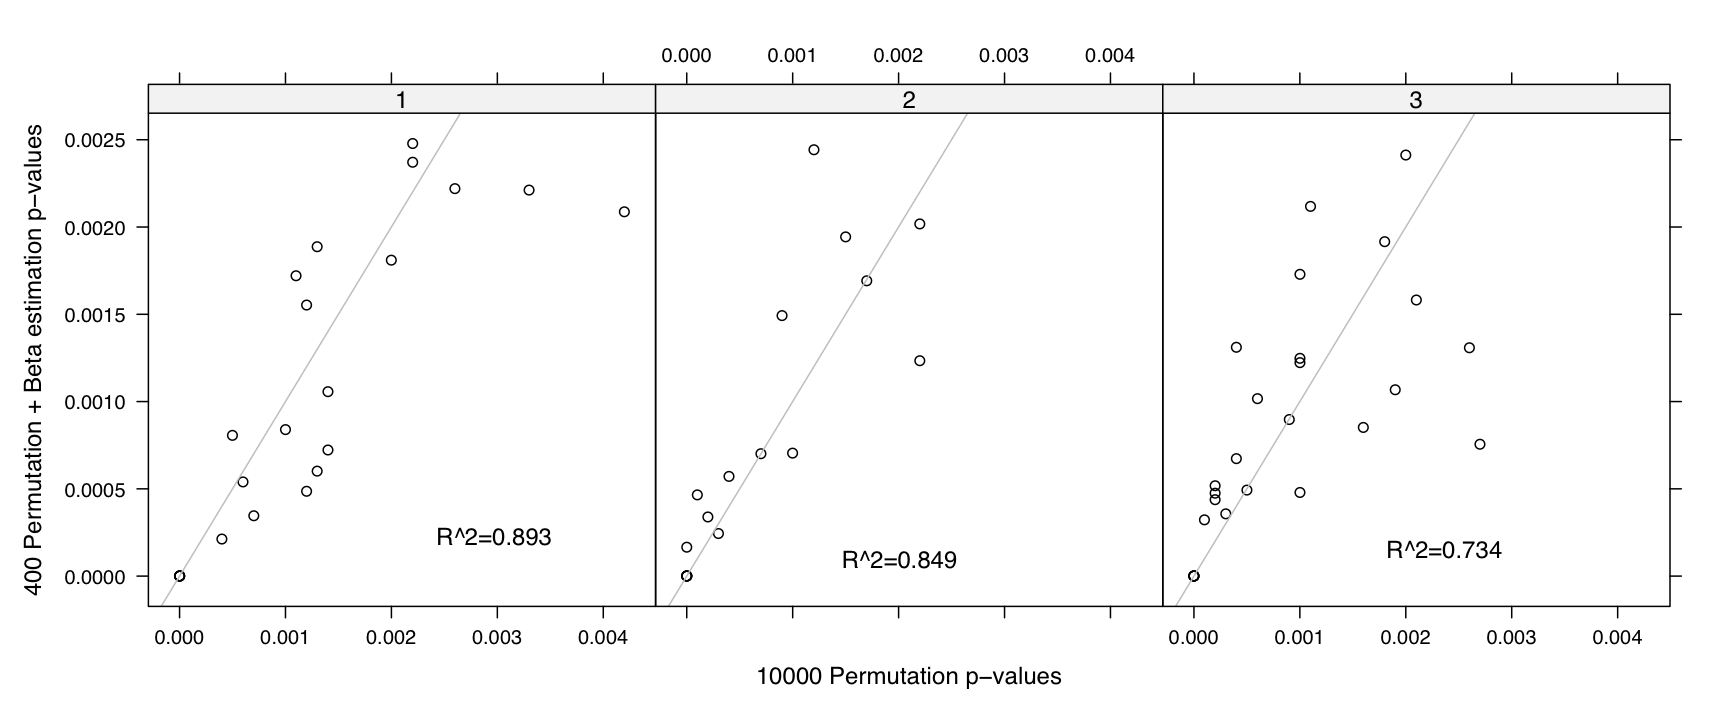
\includegraphics[width=\textwidth]{figure1.png}
          \end{column}
        \end{columns}    %--------------------------------

      \end{block}

    \end{column}

    \begin{column}{.2\linewidth}
      \begin{block}{System Overview}
        \vfill
        \noindent{\textbf{Visual Modeling (VM)}}
        \begin{itemize}
        \item related to the acoustic model in ASR
        \item HMM based, with separate GMMs, globally pooled diag. covariance matrix
        \item monophone whole-word models
        \item pronunciation handling
        \end{itemize}

        \vskip1ex
        \noindent{\textbf{Language Modeling (LM)}}
        \begin{itemize}
        \item according to ASR: LM should have a greater weight than the VM
        \item trigram LM using the SRILM toolkit, with modified Kneser-Ney discounting with interpolation
        \end{itemize}

      \end{block}

    \end{column}

  \end{columns}   %%%%%%%%%%%%%%%%%%%%%%%%%%%%%%%%%%%%%%

  \begin{columns}   %%%%%%%%%%%%%%%%%%%%%%%%%%%%%%%%%%%%%%
    \begin{column}{.45\linewidth}
      \begin{block}{Feature Selection and Model Combination}
            \noindent{\hskip1cm\textbf{Feature Selection}}\par
            \begin{itemize}
            \item \alert{concatenation} of appearance-based and manual features
            \item \alert{sliding window} for context modeling
            \item \alert{dimensionality reduction} by PCA and/or LDA
            \end{itemize}

      \end{block}
    \end{column}

    \begin{column}{.45\linewidth}
      \begin{block}{Model Combination}
            \begin{itemize}
            \item \alert{log-linear combination} of independently
              trained models
            \item profit from independent alignments (\eg performing
              well for long and short words)
            \item profit from different feature extraction approaches
            \end{itemize}
      \end{block}
    \end{column}
  \end{columns}   %%%%%%%%%%%%%%%%%%%%%%%%%%%%%%%%%%%%%%

\end{frame}

\end{document}


%%% Local Variables: 
%%% mode: latex
%%% TeX-PDF-mode: t
%%% End: 
